
\documentclass[ngerman]{scrreprt}  


\usepackage{babel}


\author{Ziad Bougrine}

\usepackage{url}
\usepackage{titling}
\usepackage{graphicx}
\graphicspath{ {./pictures/} }
\usepackage{xcolor}
\usepackage{eso-pic,lipsum}
\usepackage{biblatex}
\usepackage{lmodern}
\usepackage{algorithm}
\usepackage{algpseudocode}
\usepackage{tabularx}
\usepackage{tikz}



%import package
\usepackage{graphicx}
\graphicspath{ {./pictures/} }
\usepackage{xcolor}
\usepackage{eso-pic,lipsum}
\usepackage{biblatex}
\usepackage{lmodern}
\usepackage{algpseudocode}
\usepackage{tabularx}

\addbibresource{meinequellen.bib}
\AddToShipoutPictureBG{%
 \AtPageLowerLeft{\hspace{0.5cm} FH Aachen: \rule{2cm}{3cm}}}

\title{Blockchain- Technologie : \texttt{Analyse von Proof of Work (Bitcoin) }}
\begin{document}
  \maketitle  
  \begin{abstract}
    Hier steht eine kurze Zusammenfassung des Inhaltes, es geht hier um den Aufbau eines Artikels, insbesondere um die geeignete Gliederung.
  \end{abstract}

   \begin{abstract}
   	Hier steht eine kurze Zusammenfassung des Inhaltes, es geht hier um den Aufbau eines Artikels, insbesondere um die geeignete Gliederung.
   \end{abstract}

  \tableofcontents


\chapter{Einleitung}
Seit den späten 2000er Jahren hat sich Blockchain zu einer der disruptivsten Technologien auf dem globalen Markt für digitale Transaktionen entwickelt.\\ \\
In der Jahre 2008 wurde ein Whitepaper mit dem Titel Bitcoin: „A Peer-to-Peer Electronic Cash System“ von einer Person (oder einer Gruppe von Personen) unter dem Namen Satoshi Nakamoto veröffentlicht. Vier Monate später, am 3. Januar 2009, erstellten sie den Genesis-Block, was der Beginn und der Tag 0 des Bitcoin- und Blockchain-Netzwerks ist. Blockchain betrachtet als öffentlich verteiltes Hauptbuch für Bitcoin-Kryptowährung Transaktionen zu dienen, basierend auf die Methode „Proof-Of-Work“, um die Schaffung und den Handel von Bitcoin und anderen Kryptowährungen während der Finanzkrise 2007/08 zu unterstützen. In heutigen Tagen gibt es jetzt viele Kryptowährungen. Zum Beispiel : Litecoin(2011), Ethereum(2015), Dogecoin(2013) usw… \\ \\
Die Implementierung der Blockchain in Bitcoin machte es zur ersten digitalen Währung, die das Problem der doppelten Ausgaben ohne die Notwendigkeit einer vertrauenswürdigen Behörde löst. Einer der Hauptvorteile besteht darin, dass jeder erstellten Block, der Datensatz enthält unveränderlich ist und seine Authentizität von der gesamten Gemeinschaft autorisierter Benutzer und nicht von einer einzigen zentralen Behörde überprüft werden kann. Das System ist daher darauf ausgelegt, die Transparenz und Rechenschaftspflicht einer digitalisierten Transaktion zu verbessern. Nehmen wir ein Beispiel, um dieses Konzept gut zu verstehen. Wir haben ein Transaktionsbanksystem, von dem aus einem Server oder Systemadministrator alles verwalten kann. Dies kann die Wartung des Systems, das Verwalten, Löschen und Hinzufügen von Benutzer- oder Transaktionsinformationen zur Datenbank umfassen. Oder er sagt einfach, dass Sie ihm 10.000 € schulden, was gefährlich ist. \\ \\
Das ist der Hauptgrund, warum Blockchain-Technologie erfunden worden. Indem es immer für alle sichtbar im Hauptbuch aufgezeichnet wird, wenn Geld von einem Konto auf ein anderes überwiesen wird.



\chapter{Einführung in die Blockchain}

%##############################
%#           Section 1        #
%##############################
\section{Blockchain Definition}
\textbf{Blockchain} ist eine kontinuierlich erweiterbare Liste von Datensätzen in einzelnen Blöcken, es ist ein offenes Hauptbuch für Personen, die Datensätze sehen und erstellen können. Jeder Block besteht aus Daten, Hash, vorherigem Hash und Zeitstempel. Entscheidend ist, dass wir spätere Transaktionen auf früheren Transaktionen aufbauen können und diese als richtig bestätigen können, indem wir die Kenntnis der früheren Transaktionen beweisen können. Damit wird es unmöglich gemacht, Existenz oder Inhalt der früheren und späteren Transaktionen zu manipulieren. Andere Teilnehmer der dezentralen Buchführung erkennen eine Manipulation der Blockchain dann an der Inkonsistenz der Blöcke.\\
\\
\\
\\
\textbf{Blockchain} ist ein Distributed Ledger, diese Technologie nennt sich Self regieren (Self governing), was bedeutet, dass es nicht eine Person gibt, die kontrollieren und machen kann
ändern, stattdessen kommen Beiträge von Tausenden von Benutzern
die am Blockchain-Netzwerk teilnehmen, um es funktionsfähig zu machen. Wenn eine Person betrügt, wird sie schnell sein
als Betrug angesehen, da der Rest des Netzwerks sie überprüft.


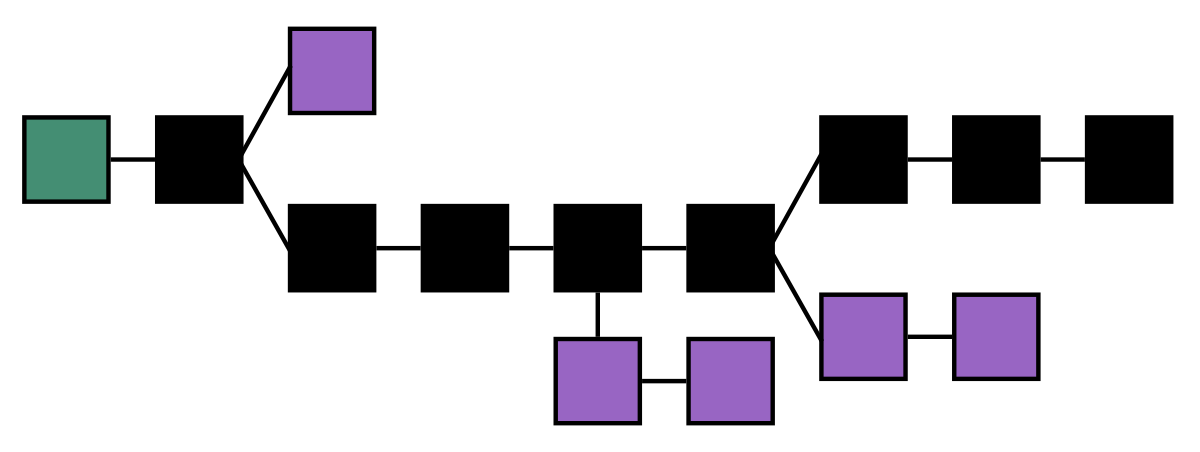
\includegraphics[width=\linewidth]{1.png}

\section{Konstruktion des Blocks}
Ein Block speichert Informationen über Transaktionen, Zeitstempel, vorherigen Hash, Block-Hash.
\begin{itemize}
\item \textbf{Magische Zahl :} Nummer, die diesen Block als Teil des Netzwerks einer bestimmten Kryptowährung identifiziert.
\item \textbf{Transaktionen :} die Hauptinformationen und auch den größten Teil des Blocks
\item \textbf{Transaktionszähler :} die Anzahl der im Block gespeicherten Transaktionen
\item \textbf{Block Größe :} die maximale Größe der Informationen, die der Block enthält
\end{itemize} 
Ein Block enthält viele Informationen, belegt jedoch nicht viel Speicherplatz. Nehmen wir diese Elemente als Beispiel:
Was ist die Hauptinformationen, die ein Block (Transaktionen) enthält?
\begin{itemize}
\item \textbf{Version:} Sie ist benutzbar, um einen neuen Block zu erstellen und um eine neue Version von Software zu identifizieren. Es ist auf 4 Bytes (4 x 8 „bits“) codiert.
\item \textbf{Vorheriger Block-Hash:} Enthält einen Hash des Headers des vorherigen Blocks (md5, sha256 ...). Es ist auf 32 Bytes (32 x 8 = 256 „bits“) codiert.
\item \textbf{Hash Merkle root:} Hash of transactions in the Merkle tree of the current block. Es ist auf 32 Bytes (32 x 8 = 256 „bits“) codiert.
\item \textbf{Time:} Erstellungszeit des Blocks. Es ist auf 32 Bytes (32 x 8 „bits“) codiert.
\item \textbf{Bits:} Es ist ein Wert, der die Schwierigkeitsbewertung des Ziel-Hashes und die Schwierigkeit beim Lösen der „Nonce“ angibt. Es ist auf 32 Bytes (32 x 8 „bits“) codiert.
\item \textbf{Nonce:} Es ist die magische Zahl, die der Miner lösen muss, um einen Block im Blockchain-Netzwerk zu verifizieren und zu schließen.\\ \\ \\ \\ \\
\end{itemize}

\color{green}
\huge{\textbf{Information :}} 
\color{black}
\normalsize
Die Miner interessieren sich für die Nonce, weil das Mining-Programm Zufallszahlen (Bruteforce) verwendet, um die Nonce im Hash zu erraten. Der Hash wird verifiziert, wenn die Nonce gelöst ist. Wenn die Nonce oder eine Zahl darunter erraten wird. Dann schließt das Netzwerk diesen Block, generiert einen neuen mit einem Header und der Prozess wiederholt sich. \\ \\ \\ \\ \\ \\

\large
\underline{\textbf{Was sind Merkle-Bäume?}} \\ \\
\normalsize
Es handelt sich um eine Datenstruktur in Form eines Binärbaums, der in Bitcoin und Kryptowährung weit verbreitet ist und zur effizienteren und sichereren Codierung von Daten verwendet wird.




\section{Blockchaining-Mechanismus}
\textbf{Der Blockchain-Mechanismus} funktioniert wie eine Linkedlist, er enthält eine Kette von Blöcken
dass jeder Block der Kette aus einem Hash dieses Blocks und einem Hash des vorherigen Blocks zusammengesetzt ist. Es ist derselbe Mechanismus wie bei der Linkedlist, da jeder Knoten der Liste einen Zeiger auf den letzten Knoten enthält. Was es ermöglicht, über die Kette zu iterieren.

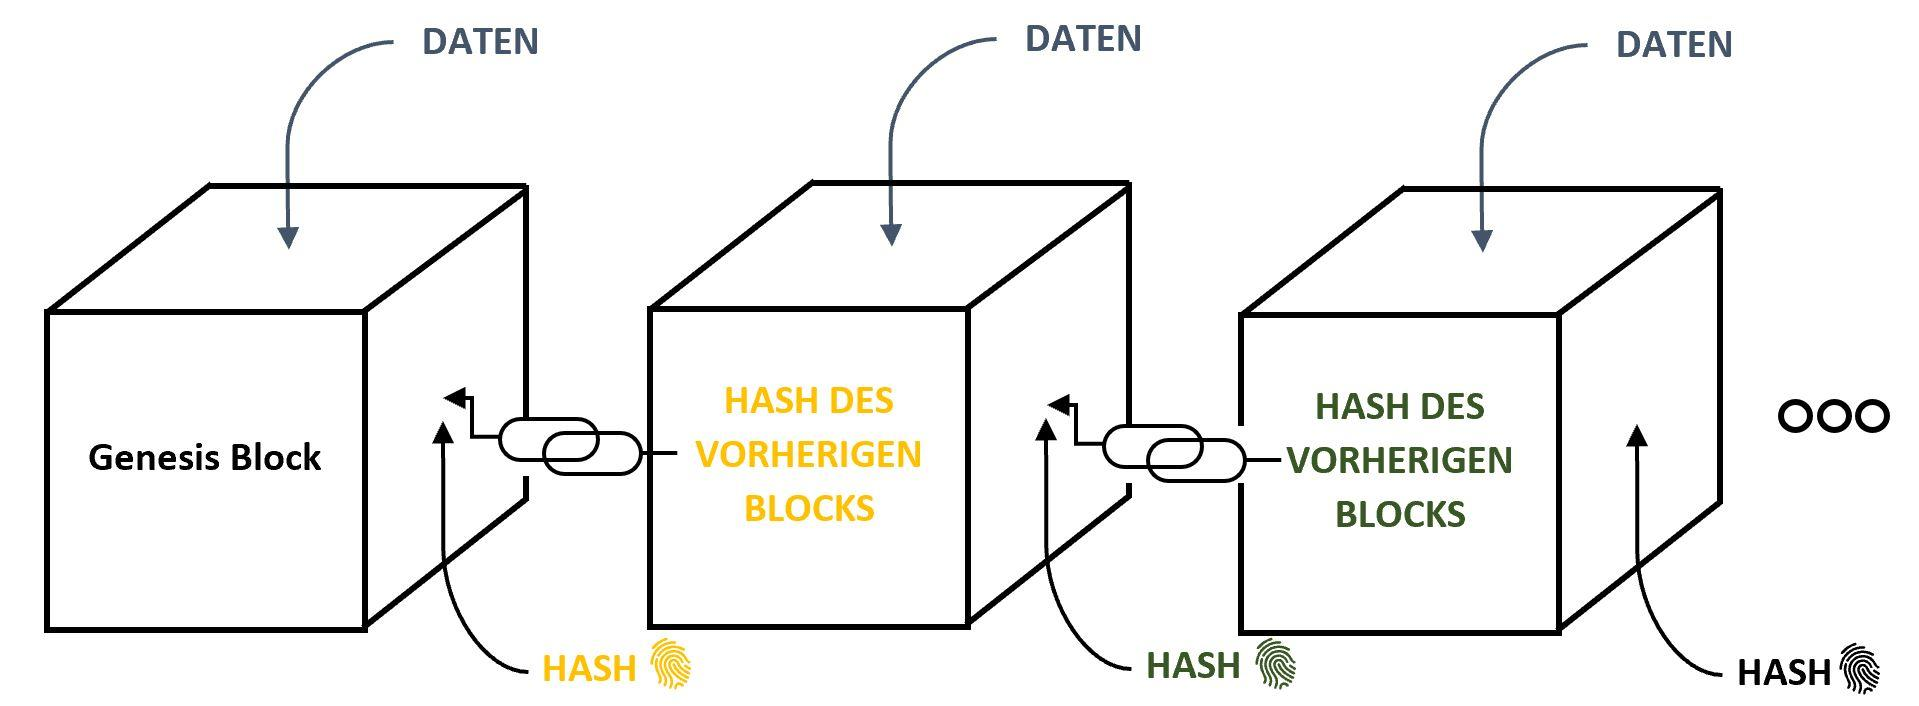
\includegraphics[width=\linewidth]{2}


\textbf{Der erste Block der Kette wird als Genius-Block bezeichnet.} \\ \\ \\


In diesen Situationen sollten wir immer darüber nachdenken, was verdächtige Personen tun könnten, sie könnten die Daten im Block (i) ändern oder manipulieren.
dies führt zu einer Modifikation des tatsächlichen Blocks i und macht den vorherigen Hash im Block (i+1) ungültig. Das bedeutet, dass das Ändern eines Blocks alle nächsten folgenden Blöcke im Blockchain-Netzwerk ungültig macht, was die Qualität der Herstellung einer Kette beweist.\\ \\ \\ 
\color{red}
\huge{\textbf{Achtung :}}
\color{black}
\large
ist dieser Mechanismus gesichert ?\\ \\
\normalsize
 	
Die Verwendung von Hashes reicht nicht aus, um Manipulationen zu verhindern. Computer sind heutzutage sehr schnell und können Tausende von Hashes berechnen. Technisch gesehen können wir einen Block manipulieren und alle nächsten Hashes der nächsten Blöcke neu berechnen, um das Blockchain-Netzwerk wieder gültig zu machen. Aus diesem Grund verwendet Blockchain Proof of Work
in diesen Fällen. Es gibt eine Möglichkeit, dieses Problem zu verhindern. Es ist der berühmte „Proof of Work (POW)“.	








\chapter[Theoretische Seite der Proof-Of-Work-Methode]{Einführung in die „Proof-Of-Work“-Methode}	

\section{Was ist Proof-Of-Work ?}
Proof-Of-Work kam mit einem Grundprinzip, wenn ein Miner versucht, einen Block zur Kette von Blöcken im Blockchain-Netzwerk hinzuzufügen, macht es diese Methode schwierig. Der Miner sollte sich viel Mühe geben, um den Block zu erstellen. Diese Methode basiert auf vielen Grundlagen der Kryptowährung wie folgt:

\begin{itemize}
	\item{Die Schwierigkeit, einen gültigen Hash zu finden, um den Block dem Blockchain-Netzwerk hinzuzufügen, ist so gewählt, dass alle zehn Minuten ein neuer Block mit einer bestimmten Anzahl von BTC in unsere Kette kommt.
		Dies sichert das algorithmische Geldmengenwachstum.}
	\item{Mit Hilfe von PoW ist es für Nodes sehr einfach zu erkennen, welche Blockchain die richtige ist: vor allem diejenige, der er die meiste Arbeit in Form von Rechenkapazität leistet.}
	\item{Proof of Work sichert das Blockchain-Netzwerk vor allen Angreifern, denn diese müssten mehr Energie in das Netzwerk einspeisen als alle anderen insgesamt verfügbaren Miner – und das über einen langen Zeitraum. Das ist beim Bitcoin unmöglich.}
	\item{Proof of Work ist ferner der fairste Mechanismus der Neuverteilung von Geld, den wir kennen. Denn im Gegensatz zu Fiatgeld können frische Coins nicht mit einem Federstrich erzeugt werden, sondern erfordern einen realen Aufwand an Ressourcen.}
\end{itemize}

\section{Wie funktioniert Proof of Work bei einer Blockchain ?}
Dieser Mechanismus von PoW wird als Mining bezeichnet, was bedeutet, die Nonce mit bestimmten Eigenschaften zu erraten, indem Milliarden von Berechnungen durchgeführt werden. Wenn Sie ein solches Ergebnis erzielt haben, erhalten Sie eine Belohnung mit der sogenannten Blocksubvention.\\ \\ \\ \\
\textbf{Diese beschreiben den Vorgang einer Transaktion im Blockchain-Netzwerk \\ }
\begin{itemize}
	\item{Das Blockchain-Netzwerk erstellt einen Block, der alle Transaktionen enthält}
	\item{Der Miner wird überprüfen, ob die Transaktionen legitim sind}
	\item{Alle Bergleute beginnen zu versuchen, die Lösung zu finden (was bedeutet, erraten Sie die Nonce), und der erste, der sie findet, erhält eine Belohnung und auch die Transaktionsgebühren}
	\item{Der Block wird der Blockchain hinzugefügt}
	\item{Der Prozess wird wiederholt \\}
	
\end{itemize}
\textbf{Dies ist ein sequentielles Diagramm, das erklärt, wie es funktioniert \\}
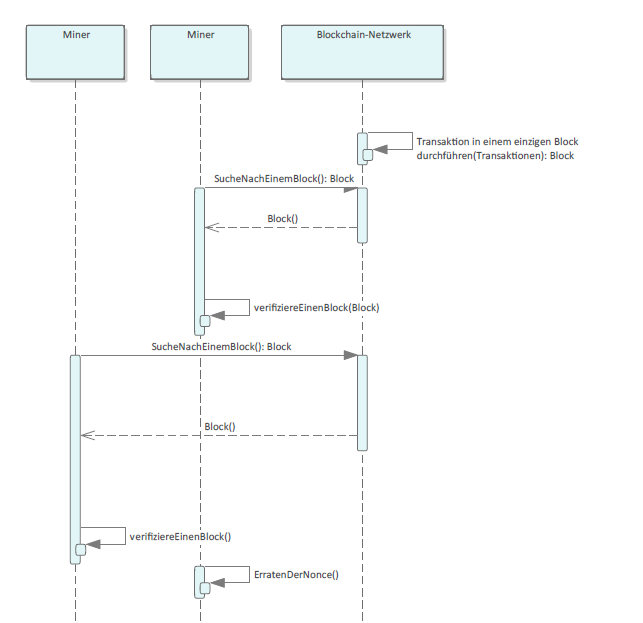
\includegraphics[width=\linewidth]{ProofOfWork1.png} \\ \\
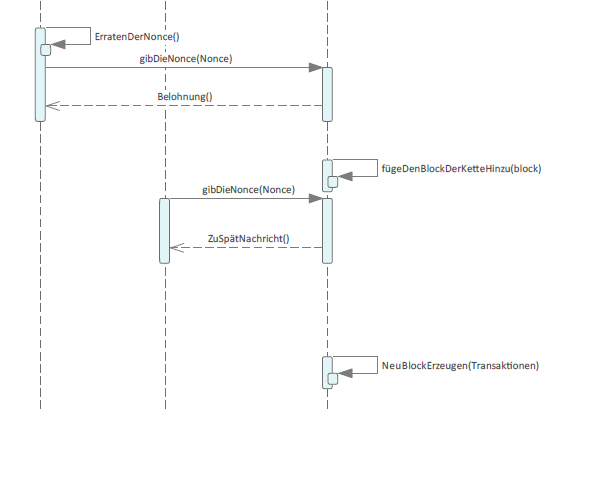
\includegraphics[width=\linewidth]{ProofOfWork2.png}
\section{Wie genau funktionieren die Proof-of-Work-Berechnungen?}
\begin{itemize}
	\item {Die Miner verwenden Hash-Funktionen. Sie sind injektive mathematische Funktionen, die nicht rückgängig gemacht werden können. Sie erzeugen aus einer beliebig langen Zeichenfolge eine eindeutige Zeichenfolge fester Länge.Die Schwierigkeit liegt darin, ein Ergebnis mit bestimmten Eigenschaften zu finden, die sich aus der Hash-Funktion ergeben. Bitcoin verwendet beispielsweise die SHA-256-Hash-Funktion für das Mining.}
	\item{Die Hash-Funktion liefert ein unvorhersehbares Ergebnis, deshalb sollten wir die Frage stellen: "Welche Zeichenfolgen müssen der Hash-Funktion übergeben werden, um einen genauen Wert zu erzeugen?". Da die bekannteste Eigenschaft der Hash-Funktion ist, dass niemand die Operation einfach umkehren kann, kann der Miner auf andere Weise die erhaltene Zeichenfolge nicht einfach umkehren und die Eingabe der Hash-Funktion erhalten.}
	\item{Aus diesem Grund gibt es das Konzept des Mining, die Miner versuchen, die Nonce und die Reihenfolge jedes Parameters zu erraten, die die Hash-Funktion als eine Zeichenfolge nimmt und ein Ergebnis liefert. Es gibt eine Billard von Operationen, die vom Bergmann durchgeführt werden, um den Wert der Eingabe zu erreichen.}
	\item{Wenn der Block abgebaut wird, überprüfen alle Teilnehmer des Blockchain-Netzwerks die präsentierte Lösung, um eine gültige Blockchain zu haben}
\end{itemize}
\section{Was hat es mit der Difficulty auf sich ?}
\begin{itemize}
\item{Die Schwierigkeit besteht darin, die gewünschte Hash-Ausgabe zu finden. Zum Beispiel Bitcoin, es wird eine Frage gestellt: Wie viele Nullen soll die Ausgabe am Anfang des Strings haben. Je mehr Nullen gefordert sind, desto schwieriger wird es schließlich, den Output zu finden.}
\item{Die Schwierigkeit ist bei Bitcoin immer so gewählt, dass im Schnitt alle zehn Minuten ein neuer Block gefunden werden soll. Dieser Benchmark wird alle zwei Wochen überprüft. Stellt sich heraus, dass in zwei Wochen der Richtwert von 2.016 Blöcken überschritten wurde, also mehr Blöcke als gewünscht gefunden wurden, ist die Schwierigkeit zu gering und wird nach oben korrigiert – und umgekehrt. (check it)}
\end{itemize}

\section{This is the algorithm side}
\begin{itemize}
	\item[--] Jetzt möchte ich darüber sprechen, wie der Arbeitsnachweis technisch funktioniert, sehen wir uns zuerst eine echte Blockstruktur von der offiziellen Website „blockchain.com“ an. \\
	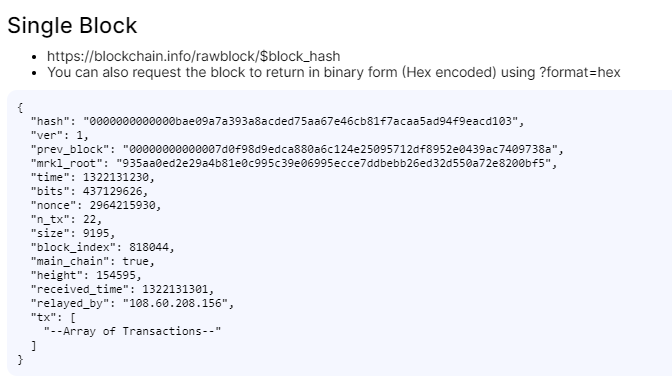
\includegraphics[width=\linewidth]{realblock.png} \\
	\item[--] Und dies ist eine echte Einzeltransaktionsstruktur \\
	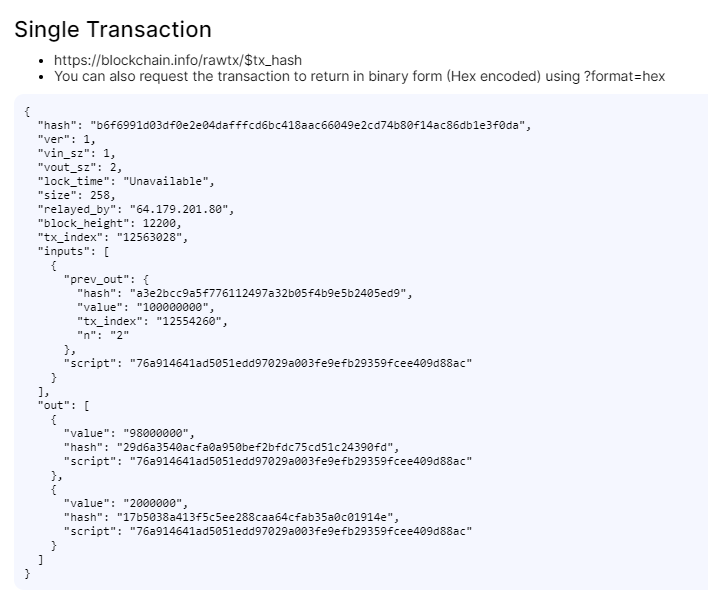
\includegraphics[width=\linewidth]{realtransaction.png} \\ \\
	\item[--] Das nächste Klassendiagramm zeigt die gesamten Daten aus dem realen Blockchain-Netzwerk. Es ist gut, es in Form eines Klassendiagramms zu sehen, um zu erkennen, wie Daten für die Implementierung miteinander in Beziehung stehen \\
	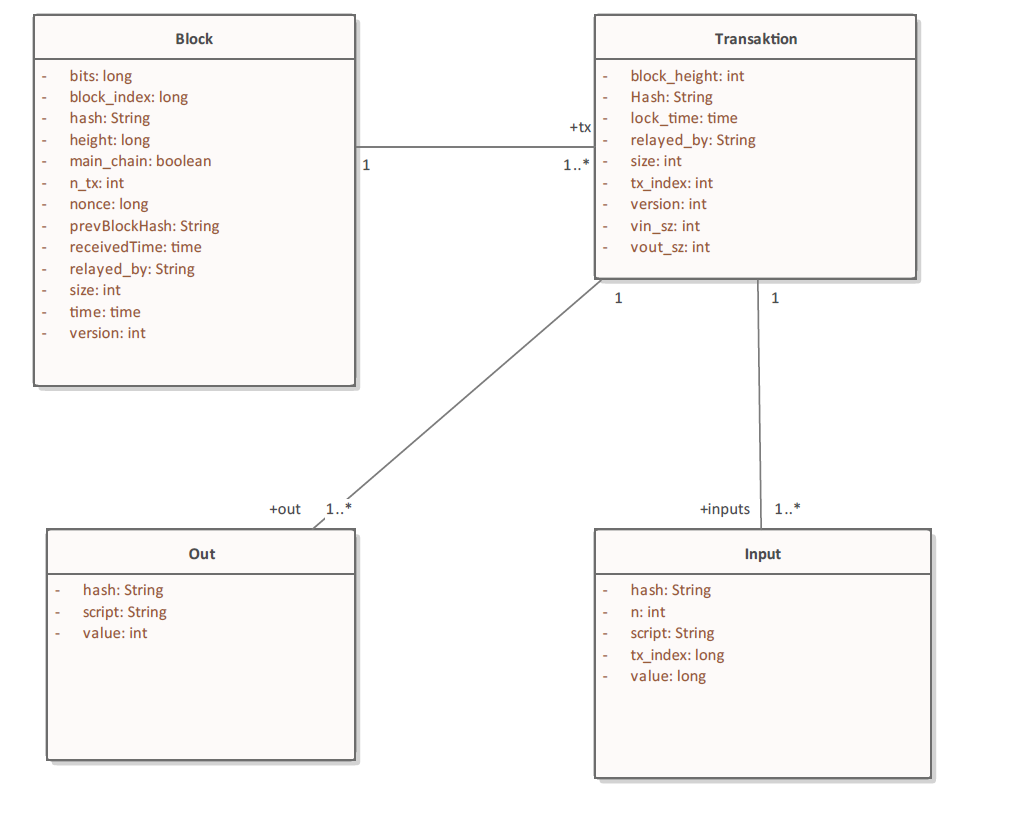
\includegraphics[width=\linewidth]{classOfStructures.png} \\ \\
	\item[--] {Und jetzt erklären wir unseren Algorithmus mit dem Aktivitätsdiagramm, zuerst sollten wir Daten initialisieren, die Initialisierung von Max\textunderscore Nonce \textunderscore Limit, Anzahl der Nullen, für dieses Beispiel werden wir berücksichtigen, dass der Hash mit 4 Nullen beginnen sollte (nur für Informationen, Anzahl von Nullen sind wichtig, es zeigt die Komplexität des Algorithmus, wenn die Zahl hoch ist wie 7 oder 6 Nullen, wird es ein Jahr dauern, die Nonce mit wenig Hardware-Material zu finden.Wir sollten auch unsere i-Inkrement-Variable für die for-Schleife initialisieren } \\ \\
		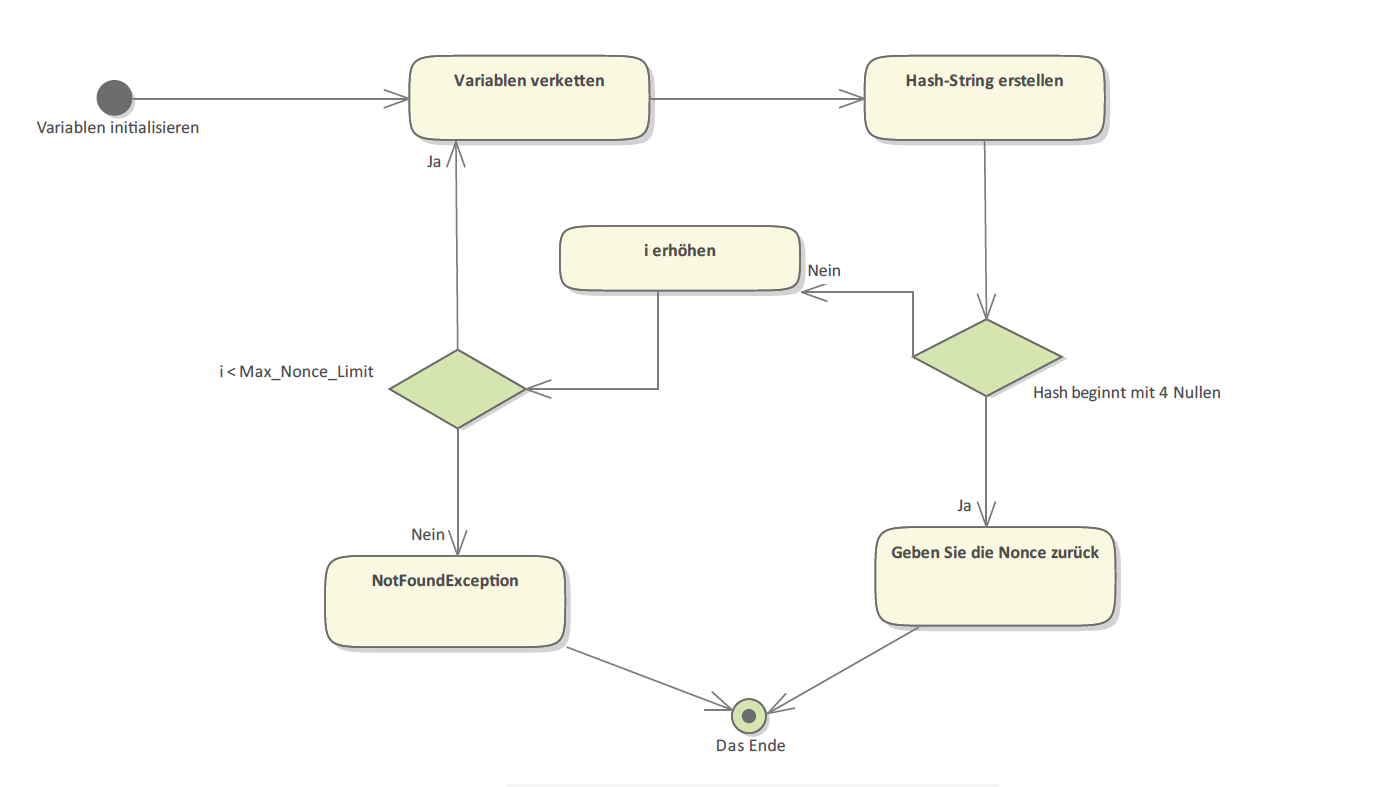
\includegraphics[width=\linewidth]{activity.png} \\ \\
		

	
\end{itemize}
\begin{LARGE}
	\textbf{Dies ist der Algorithmus \textcommabelow der für dieses Beispiel zum Schürfen von Bitcoin geschrieben wurde} \\
\end{LARGE}
\begin{algorithmic}
	\State $i \gets 1$
	\State $MaxNonceLimit \gets 100000000$
	\State $zeros \gets 4$
	\For{$i \ensuremath{<} MaxNonceLimit$}
		\State $data \gets blockNumber + transactions + prvHash + i$
		\State $hashVariable \gets  SHA256(data)$
		\If {$hashVariable.startWith(\textquotesingle 0 \textquotesingle \textasteriskcentered 4)$}
			\Return $i$
		\EndIf
	\EndFor
	
\end{algorithmic}

\section{Sicherheit des Proof-Of-Work}

\section{Vor- und Nachteile von Proof-Of-Work}
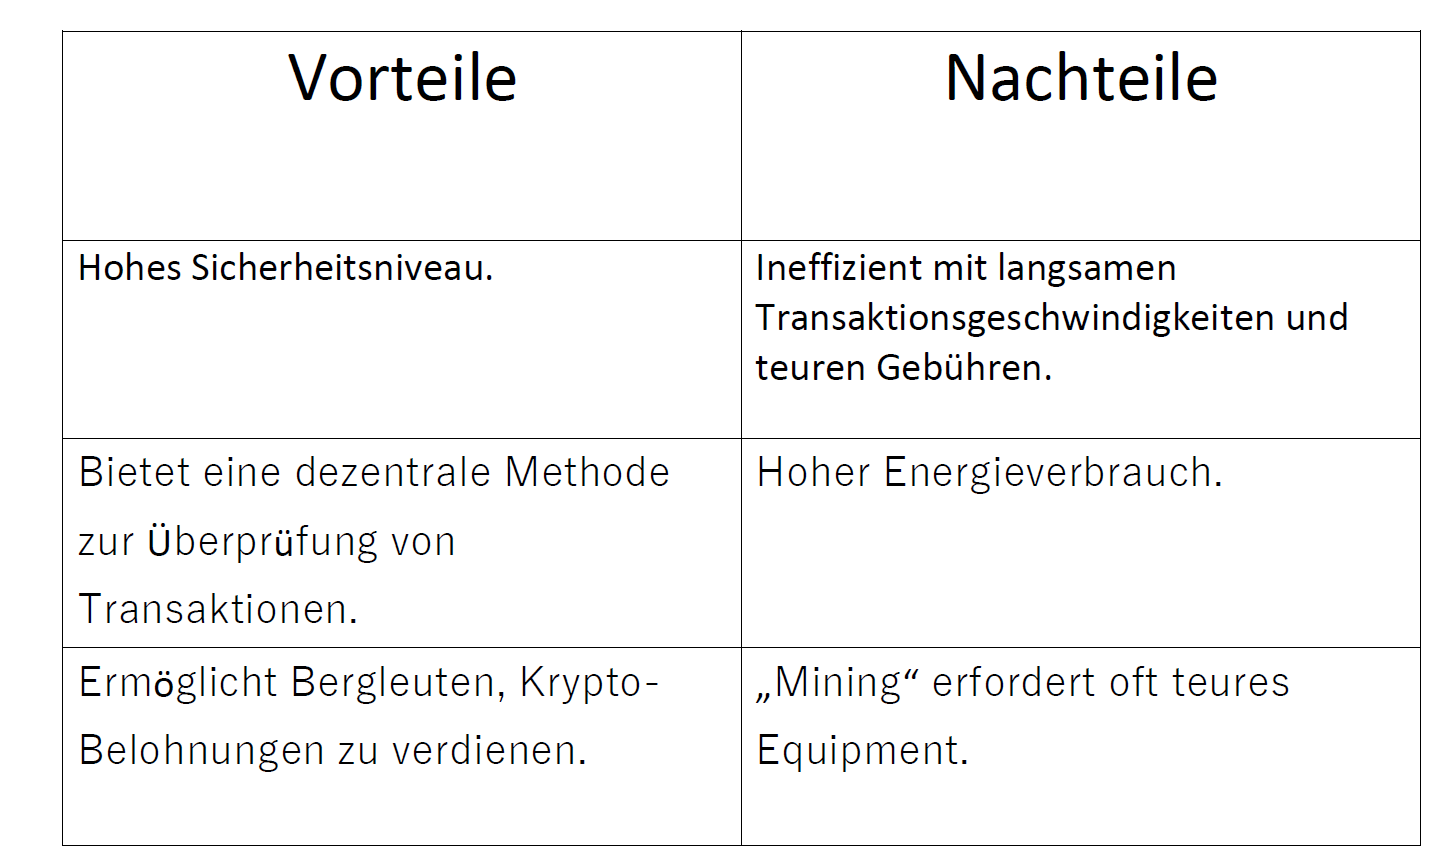
\includegraphics[width=\linewidth]{vornach.png} \\ \\



\chapter{Der Bitcoin-Markt und die Verwendung von Proof of Work}
\section{Münzen}

\begin{itemize}
	\item[--] Bevor ich anfange, mit Ihnen darüber zu sprechen, wie Sie mit Bitcoin Geld verdienen können, möchte ich Ihnen zunächst einige Münzen vorstellen, die die Proof-Of-Work-Methode verwenden
	\begin{itemize}
		\item [--] {Bitcoin Cash} \\ \\ 
		
\includegraphics[width=5cm,height=5cm]{bitcoincash.png}\\ \\
		
		\item [--] {Bitcoin SV} \\ \\
		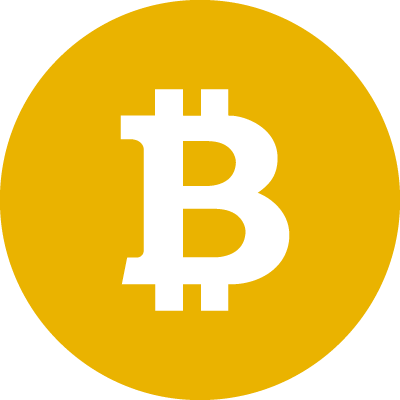
\includegraphics[width=5cm,height=5cm]{bitcoinsv.png}\\ \\
		\item [--] {Litecoin} \\ \\ 
		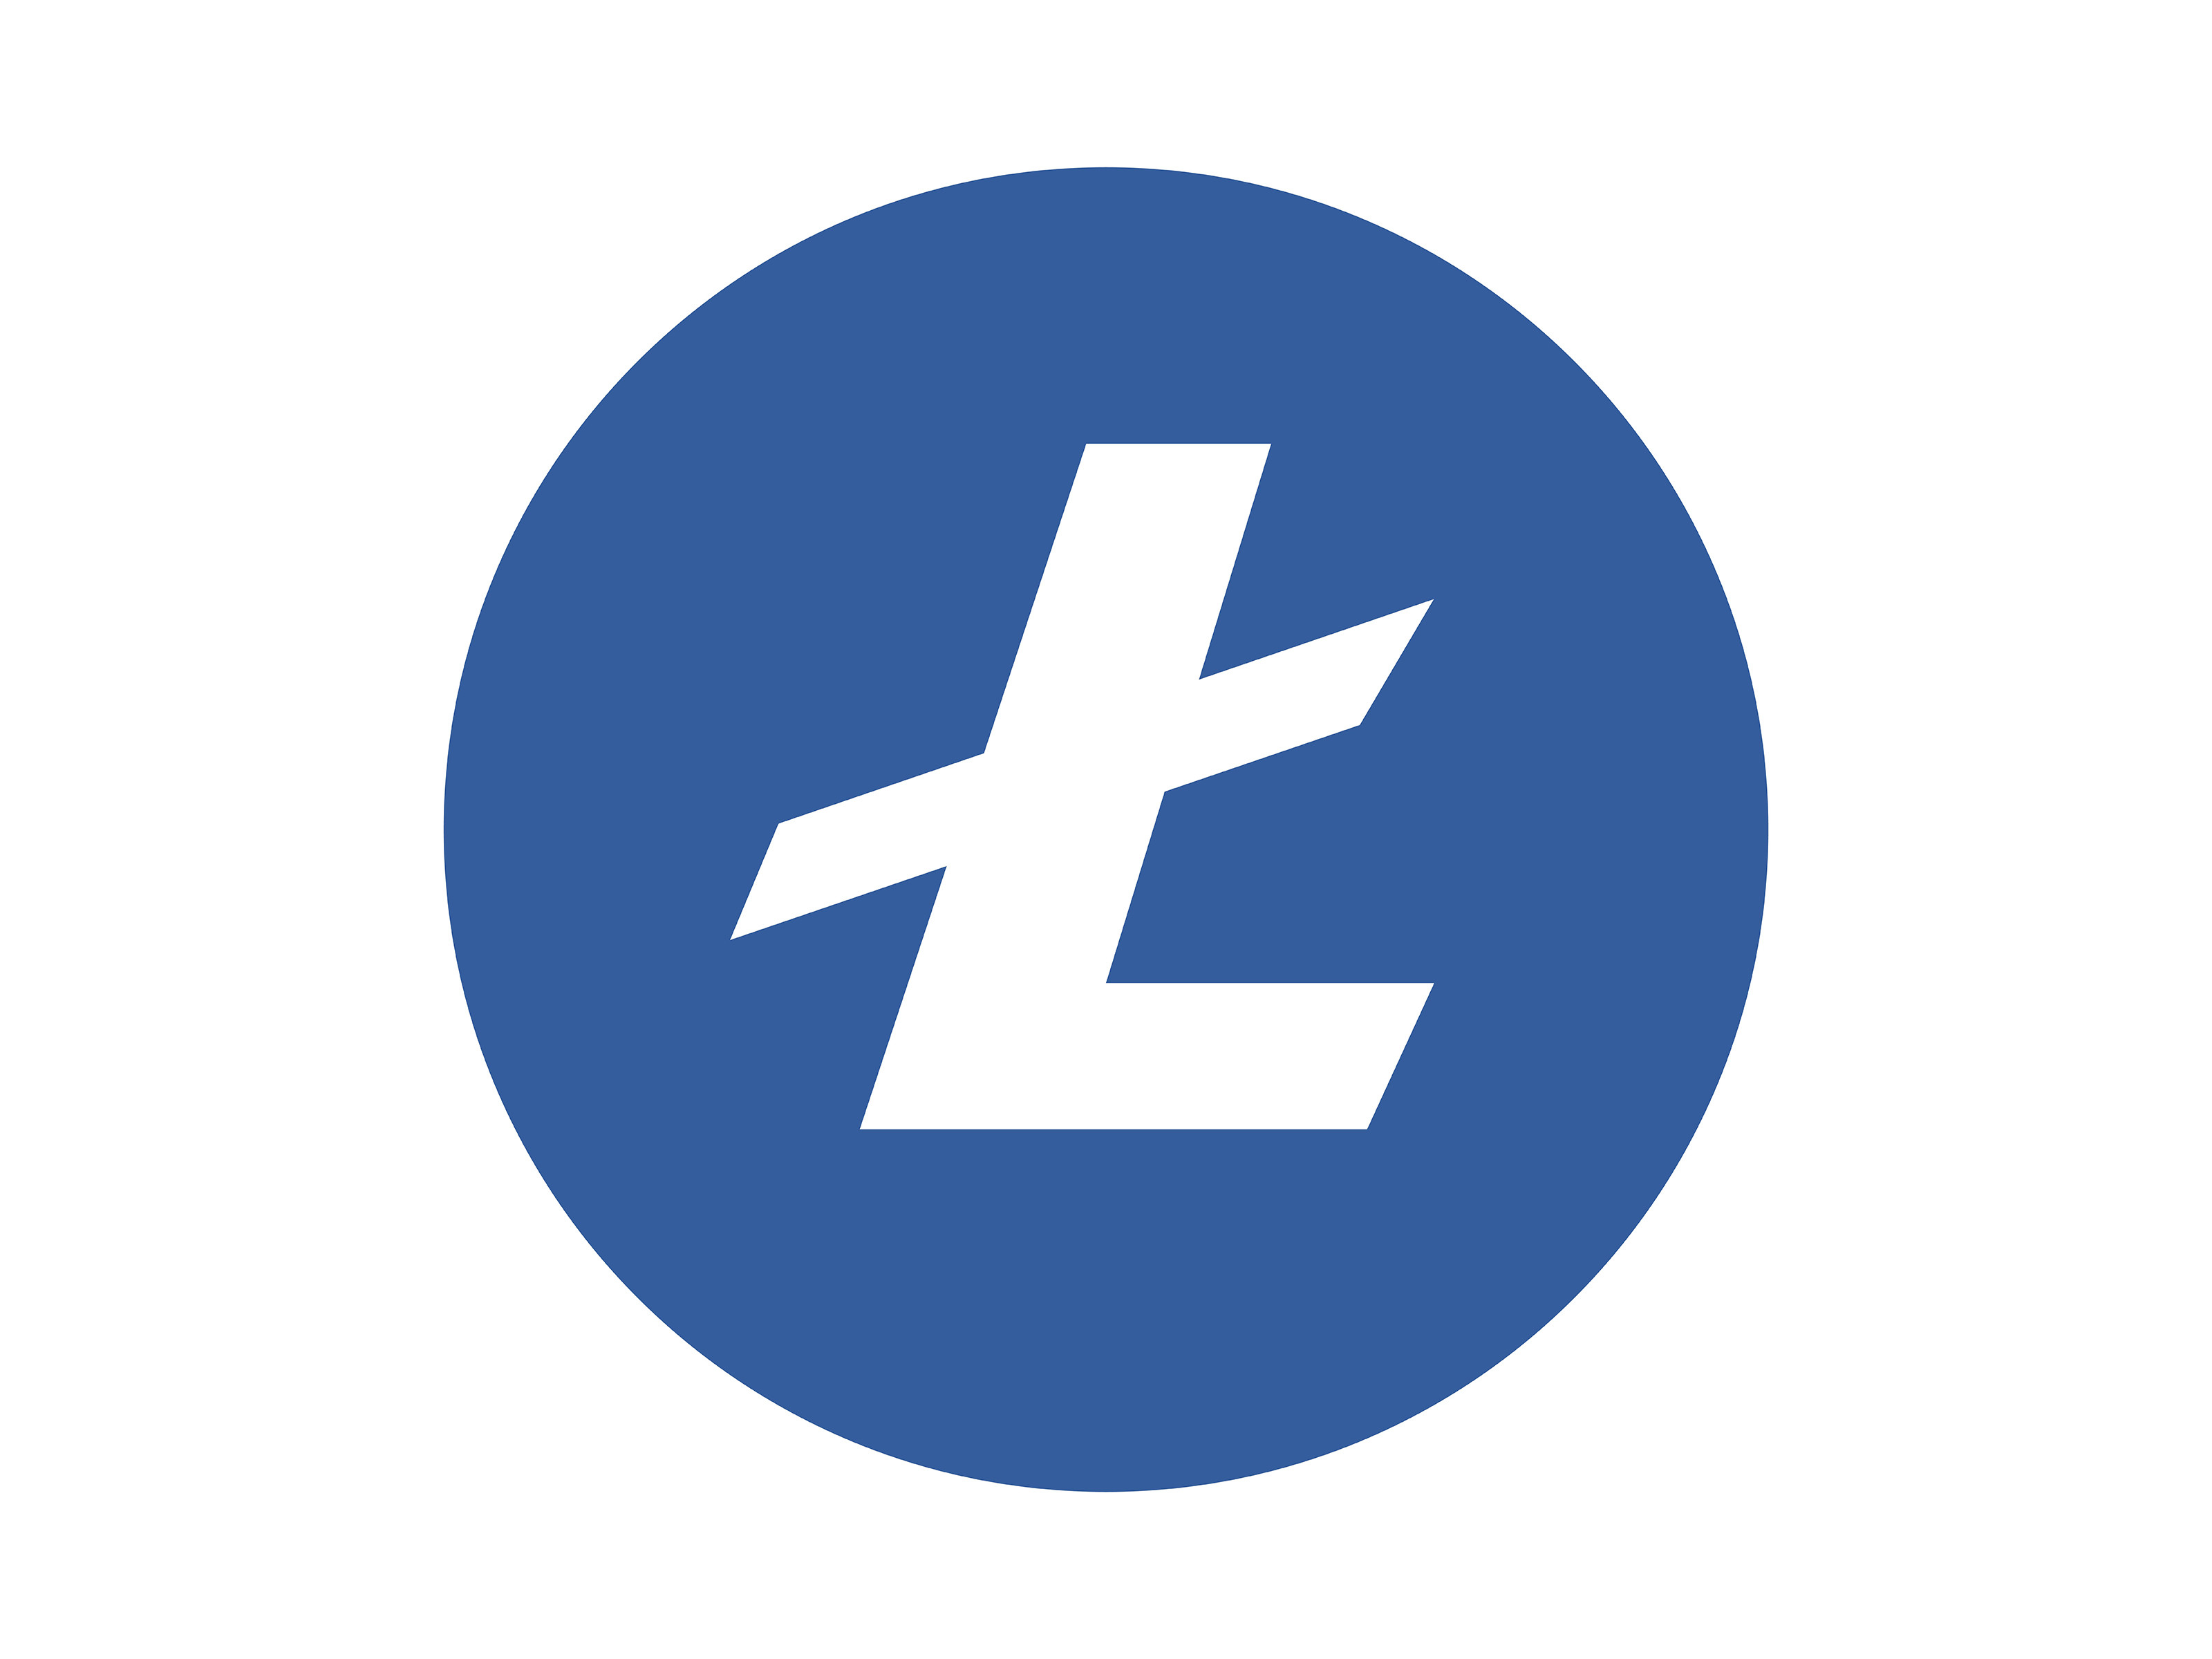
\includegraphics[width=5cm,height=5cm]{litecoin.jpg} \\ \\
		\item [--] {Dogecoin} \\ \\
		
\includegraphics[width=5cm,height=5cm]{dogecoin.png}\\ \\
		\item [--] {Bitcoin Gold}\\ \\
		
\includegraphics[width=5cm,height=5cm]{bitcoingold.png}\\ \\



	\end{itemize}
	
	\item[--] Es gibt auch viele andere Kryptowährungen, die nicht auf Bitcoin basieren, aber die Proof-of-Work-Methode verwenden :
	\begin{itemize}
		\item{Ethereum Classic}\\ \\
		
\includegraphics[width=5cm,height=5cm]{ethereumclassic.png}\\ \\
		\item{Monero}\\ \\
		
\includegraphics[width=5cm,height=5cm]{monero}\\ \\
		\item{Zcash}\\ \\
		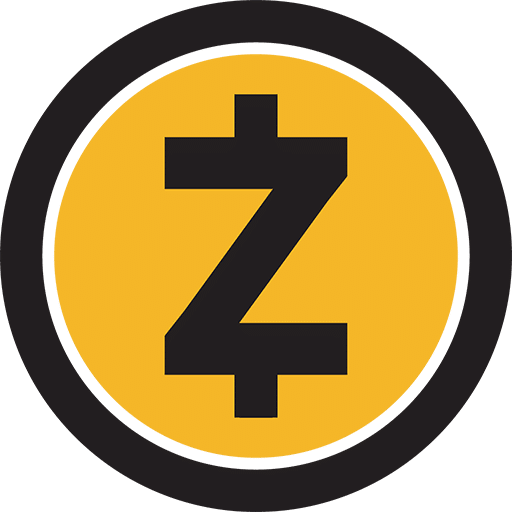
\includegraphics[width=5cm,height=5cm]{zcash}\\ \\
		\item{Kadena}\\ \\
		
\includegraphics[width=5cm,height=5cm]{kadena}\\ \\
		\item{Ravencoin}\\ \\
		
\includegraphics[width=5cm,height=5cm]{Ravencoin}\\ \\
		\item{Siacoin}\\ \\
		
\includegraphics[width=5cm,height=5cm]{siacoin}\\ \\
		\item{Horizen}\\ \\
		
\includegraphics[width=5cm,height=5cm]{horizen}\\ \\
		\item{DigiByte}\\ \\
		
\includegraphics[width=5cm,height=5cm]{digibyte}\\ \\
	\end{itemize}
\end{itemize}


\section{Wie kann ich mit Kryptowährung Geld verdienen ?}
\subsection{Krypto-Mining}
\subsubsection{Hardware}
\subsubsection{Konzept}
\subsection{Wie kann ich mein geld anlegen ?}
\chapter{Schluss}
Proof of work is a consensus mechanism used to confirm that network participants, called miners, calculate valid alphanumeric codes — called hashes — to verify bitcoin transactions and add the next block to the blockchain. It does so by having other participants in the network verify that the required amount of computing power was used by the miner that is credited with calculating the valid hash. The more miners working to verify transactions (and the faster they can generate hashes), the higher a network's hash rate.


\chapter{Literatur}
\begin{itemize}
	\item Section 1

	\item 
	
\end{itemize}
\end{document}
